\chapter{Elementary Number Theory: Primes, Congruences, and the Mechanisms of Integers}

\section{A Class That Will Not Split: Starting with a Line-Up}

At the school sports day, the PE teacher wants to arrange the second-year middle-school pupils in rows, with equally many in each row and nobody left over. Three sixth-grade classes report their numbers: Class A has $48$ pupils, Class B has $45$, and Class C has $47$.

Class A sorts itself out quickly: $48$ pupils can form $6$ rows and $8$ columns, or $4$ rows and $12$ columns, with plenty of other options. Class B has no trouble either: $45$ pupils can form $5$ rows and $9$ columns. Class C tries for ages: $2$ per row? One left over. $3$ per row? One left over. $4$, $5$, $6$ per row... always one left over. The number $47$ is like an unbreakable stone: it cannot be split into a product of two smaller integers.

Make an intuitive guess first: are these ``stone numbers'' rare oddities, or are they scattered everywhere? Do they eventually run out---could every integer beyond some point be breakable? It sounds like a child's casual question while counting, yet it has challenged some of history's sharpest minds. In this chapter, we start with this ``stone'' and explore the mechanisms hidden inside integers.

\section{A First Attempt: Sieves and Misconceptions}

When $47$ refuses to split, the simplest approach is to try possible factors one by one. $2$ fails ($47$ is odd), $3$ fails ($4+7=11$ is not a multiple of $3$), and $5$ fails (the last digit is neither $0$ nor $5$). What about $7$? $7\times 6=42$ and $7\times 7=49$, so that fails too. We can actually stop here---why? Because $7\times 7=49$ already exceeds $47$. If $47$ were a product of two integers both greater than $1$, at least one would be no larger than its square root, $\sqrt{47}\approx 6.9$. Testing up to $6$ is enough; there is no need to reach $46$. This is our first mechanism: to test whether a number can be split, we need only check up to its square root.

Following this idea, someone makes a bold conjecture: ``The unbreakable numbers are the odd numbers.'' That sounds reasonable: surely every even number has a factor of $2$? But someone immediately objects: $9$ is odd, yet equals $3\times 3$; $15$, $21$, and $25$ all split too. Conversely, $2$ is even but cannot be split. Evidently, parity and factorability are different matters.

\begin{fanli}
``All odd numbers are unbreakable'' is false. $9=3\times3$, $15=3\times5$, and $21=3\times7$ are odd, yet each is a product of smaller integers. The only reliable way to decide whether a number can be split is to check every possible factor up to its square root, not to inspect its final digit or parity.
\end{fanli}

Over two thousand years ago, ancient Greek mathematicians devised a systematic method now called a ``sieve'': write out the numbers from $2$ to $100$, circle $2$, and cross out all multiples of $2$; find the next uncrossed number, $3$, circle it, and cross out all multiples of $3$; then find $5$, $7$, and so on. Every crossed-out number is a ``composite product'' divisible by something smaller; the survivors are the unbreakable stones. The method is laborious but honest: it guarantees that nothing is missed.

There is another easily overlooked shortcut: after crossing out multiples of $7$, we can stop. By the square-root bound, every composite number up to $100$ has a prime factor no larger than $\sqrt{100}=10$, so it was already eliminated when we crossed out multiples of $2,3,5,7$. Every survivor after these four rounds must be unbreakable. Sieving the numbers up to $100$ leaves this list:

\begin{center}
\begin{tabular}{rrrrr}
\toprule
$2$ & $3$ & $5$ & $7$ & $11$\\
$13$ & $17$ & $19$ & $23$ & $29$\\
$31$ & $37$ & $41$ & $43$ & $47$\\
$53$ & $59$ & $61$ & $67$ & $71$\\
$73$ & $79$ & $83$ & $89$ & $97$\\
\bottomrule
\end{tabular}
\end{center}

Count them: there are $25$. Look at the table for a while and questions emerge. Why is every entry except $2$ odd? Why do the gaps seem to widen farther down the list? Why are some close together ($41$ and $43$), while others are far apart? We will soon return to these questions one by one. Some have answers; others still do not.

\section{Inventing a Concept: Primes Are the ``Atoms'' of Integers}

The numbers that survive the sieve deserve an official name.

\begin{dingyi}[Prime and composite numbers]
An integer greater than $1$ with no positive divisors other than $1$ and itself is called a \emph{prime number} (or simply a prime); otherwise it is called a \emph{composite number}. The number $1$ is neither prime nor composite.
\end{dingyi}

The question most likely to catch us out is: ``Why exclude $1$ from the primes? Isn't $1$ divisible only by $1$ and itself?'' This is a genuinely good question. The answer lies not in the definition itself, but in a theorem to come: mathematicians want every integer to have a unique factorisation. If $1$ were prime, then $6$ could be written as $2\times3$, $1\times2\times3$, $1\times1\times2\times3$, and so on, destroying uniqueness. Excluding $1$ gives the multiplicative world of integers a clean fundamental law. Definitions are not handed down from heaven; they are carefully designed to make theorems elegant.

\begin{shuyu}{Prime number}
\textbf{Intuition}: An unbreakable ``atom'' in the integer world, made only from $1$ and itself, not from a product of smaller integers.

\textbf{Formal definition}: An integer greater than $1$ whose only positive divisors are $1$ and itself.

\textbf{Example}: $47$ is prime because none of $2,3,5$ divides it, and $7>\sqrt{47}$, so testing can stop there.
\end{shuyu}

Chemists discovered that matter consists of just over a hundred kinds of atoms; number theorists discovered that every integer greater than $1$ is ``built'' from primes. $48=2\times2\times2\times2\times3$, $45=3\times3\times5$, while $47$ is itself an atom. More remarkably, there is only one way to build each number.

\begin{dingli}[Fundamental theorem of arithmetic]
Every integer greater than $1$ can be uniquely factored into a product of primes: apart from the order in which the primes are written, the factorisation is unique.
\end{dingli}

First consider existence, which is almost as natural as a tree growing. Take any composite number and split it into two smaller numbers; if either is still composite, keep splitting. Each split strictly decreases the numbers, and integers cannot decrease forever, so the process must stop. The numbers at its ends cannot be split any further: they are primes. The diagram shows a factor tree for $360$.

\begin{center}
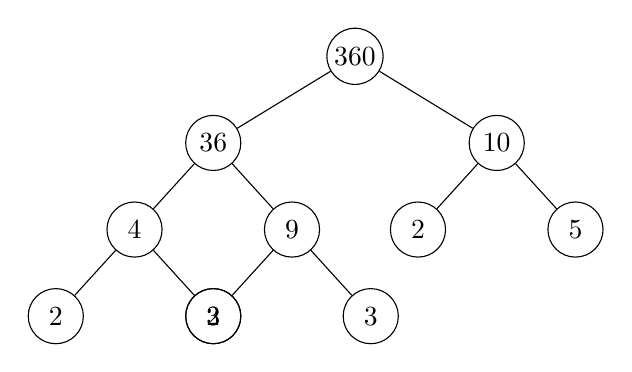
\begin{tikzpicture}[level distance=11mm,
  level 1/.style={sibling distance=36mm},
  level 2/.style={sibling distance=20mm},
  every node/.style={circle,draw,inner sep=1.5pt,minimum size=7mm}]
\node {360}
  child { node {36}
    child { node {4}
      child { node {2} }
      child { node {2} } }
    child { node {9}
      child { node {3} }
      child { node {3} } } }
  child { node {10}
    child { node {2} }
    child { node {5} } };
\end{tikzpicture}
\end{center}

Multiply all the ``leaves'': $360=2^3\times 3^2\times 5$. Take another route (perhaps starting with $12\times 30$), and the leaves are the same primes, merely encountered in a different order.

Uniqueness takes more thought. Why cannot two completely different collections of primes have exactly the same product? The key is the following lemma:

\begin{tuilun}[Prime divisor lemma]
If a prime $p$ divides a product $ab$, then $p$ divides $a$ or $b$.
\end{tuilun}

This is false for composite numbers ($6$ divides $3\times 4=12$, but $6$ divides neither $3$ nor $4$). Its proof uses the greatest common divisor from the next section, so we leave the proof idea there for now. With the lemma, uniqueness is straightforward. Suppose a number has two prime factorisations and write them on opposite sides of an equality. The first prime on the left divides the product on the right; by the lemma, it divides one of the primes on the right. Since a prime is divisible only by itself and $1$, these must be the same prime. Cancel it from both sides and repeat for what remains. Eventually, the primes on both sides must match exactly. Our intuition that ``there is only one factorisation'' is correct, and now rigorously proved.

\section{Repeated Division: A Two-Thousand-Year-Old Machine}

Now we supply the tool that the lemma was waiting for. Given two integers, say $252$ and $105$, what is the largest factor they share? This is called their greatest common divisor. The cumbersome method lists all divisors of each number and finds the intersection. But an astonishingly fast old method, recorded in ancient Greek mathematics books over two thousand years ago, still runs inside your phone's chips today.

\begin{dingyi}[Greatest common divisor]
The largest common divisor of integers $a$ and $b$ (not both $0$) is denoted by $\gcd(a,b)$. If $\gcd(a,b)=1$, then $a$ and $b$ are called \emph{coprime}.
\end{dingyi}

\begin{shiyan}
Take a sheet of paper and calculate $\gcd(252,105)$. First, divide $252$ by $105$: quotient $2$, remainder $42$. Write $252=2\times105+42$. Next, divide the previous divisor $105$ by the previous remainder $42$: $105=2\times42+21$. Finally, divide $42$ by $21$: $42=2\times21+0$. The remainder is $0$, so stop. The last nonzero remainder, $21$, is the answer: $\gcd(252,105)=21$. Just three divisions, without needing to know any factors of $252$ or $105$.
\end{shiyan}

This is the Euclidean algorithm, or repeated division. Why does it work? Its core is one statement: if $a=bq+r$, then the common divisors of $a$ and $b$ are exactly the common divisors of $b$ and $r$. Any common divisor of $b$ and $r$ must divide $bq+r=a$; conversely, any common divisor of $a$ and $b$ must divide $a-bq=r$. The collection of common divisors is unchanged, so its largest member is unchanged too:
\[
\gcd(a,b)=\gcd(b,r).
\]
The numbers on the right get smaller. The remainders decrease but cannot fall below $0$, so after finitely many steps the remainder must be $0$, and the smaller number at that stage is the answer. No prime factorisation is needed. This is precisely its strength, because factoring large integers is difficult (a fact that will later come to cryptography's rescue).

The algorithm has a beautiful geometric version. Tile a $252\times 105$ rectangle with the largest squares that fit. First place two $105\times 105$ squares, leaving a $42\times 105$ strip. Tile that strip with $42\times 42$ squares: two fit, leaving $42\times 21$. Finally, $21\times 21$ squares fill the remainder exactly. The final squares fit without any leftover edges, and their side length is the greatest common divisor. The uncovered portion shrinks just as the remainders shrink.

There is a by-product: reading the divisions backwards expresses the greatest common divisor as an ``integer linear combination'' of the original numbers. In our example:
\[
21=105-2\times42=105-2\times(252-2\times105)=5\times105-2\times252.
\]
In general, there are always integers $x,y$ such that $\gcd(a,b)=ax+by$. Do not underestimate this line: the previous section's prime divisor lemma depends on it. Suppose a prime $p$ divides $ab$ but not $a$. Then $\gcd(p,a)=1$ (the only positive divisors of $p$ are $1$ and $p$), so integers $x,y$ satisfy $px+ay=1$. Multiplying by $b$ gives $pbx+aby=b$. The first term on the left is clearly divisible by $p$, and by assumption $ab$ in the second term is also divisible by $p$. Therefore $b$ is divisible by $p$. The lemma is proved, tightening the final screw in the fundamental theorem of arithmetic.

The greatest common divisor also has an everyday use: reducing fractions. To put $\frac{252}{105}$ in lowest terms, divide numerator and denominator by $\gcd(252,105)=21$, obtaining $\frac{12}{5}$ in one step, without repeated trial cancellations. Its partner is the least common multiple: for two integers, the least common multiple times the greatest common divisor equals their product, $\mathrm{lcm}(a,b)\cdot\gcd(a,b)=ab$. Thus the least common multiple of $252$ and $105$ is $252\times105\div21=1260$. Here is where it appears: two neon lights flash every $252$ seconds and every $105$ seconds respectively. After flashing together, they next coincide exactly $1260$ seconds later. All such ``meeting again'' problems---gears realigning, planets lining up again, or two buses arriving together---have this same number behind them.

\section{Parity, Invariants, and Congruence: Another View of Integers}

Factorisation concerns multiplicative structure. Now change perspective: instead of asking which number something is, ask which class it belongs to. The simplest classification is odd or even: remainder $1$ or $0$ on division by $2$. Do not dismiss this as too simple; it is a powerful weapon, formally called an \emph{invariant}.

A classic scene: remove two diagonally opposite squares from an $8\times8$ chessboard. Can $31$ dominoes of size $1\times2$ tile what remains? You could spend an afternoon trying, always nearly succeeding. A mathematician does not try placements, but looks at colours. Every domino, horizontal or vertical, covers one black and one white square, so a tileable region must have equal numbers of each. The two removed corners have the same colour, leaving two more black squares than white, or vice versa. $31$ dominoes cover $31$ black and $31$ white squares, never $30$ and $32$. Without a single attempt, the answer is ``impossible''. Parity remains unchanged during tiling; that invariance settles the matter.

Parity is the remainder on division by $2$. Extending this idea to division by any number gives one of number theory's most useful tools.

\begin{dingyi}[Congruence]
Let $m$ be a positive integer. If integers $a$ and $b$ leave the same remainder when divided by $m$ (equivalently, if $m$ divides $a-b$), we say that $a$ and $b$ are \emph{congruent modulo $m$}, written
\[
a\equiv b\pmod{m}.
\]
\end{dingyi}

\begin{shuyu}{Congruence}
\textbf{Intuition}: Arithmetic on a clock face. It is $3$ in the afternoon; what time will it be in $14$ hours? $3+14=17$ and $17\equiv5\pmod{12}$, so it will be $5$ in the morning. On the clock face, $17$ and $5$ occupy the same position.

\textbf{Formal definition}: $a\equiv b\pmod{m}$ if and only if $m$ divides $a-b$.

\textbf{Example}: $100\equiv2\pmod{7}$, so the weekday $100$ days from today depends only on $2$: count two days ahead.
\end{shuyu}

The beauty of congruence is that it behaves much like equality: we can add, subtract, or multiply both sides by the same integer. When dealing with enormous numbers, we can therefore replace them whenever convenient by smaller stand-ins modulo $m$. Want the last digit of $7^{100}$? The last digit is the remainder modulo $10$. Since $7^2=49\equiv9\pmod{10}$ and $7^4\equiv9^2=81\equiv1\pmod{10}$,
\[
7^{100}=(7^4)^{25}\equiv 1^{25}=1\pmod{10}.
\]
The final digit is $1$. We never calculated the eighty-odd-digit giant $7^{100}$, yet we know its last digit. That is the power of looking only at classes.

Congruence also explains familiar rules whose reasons you may never have considered. For example: ``A number is divisible by $3$ if and only if its digit sum is divisible by $3$.'' Why do the digits cooperate? The secret is $10\equiv1\pmod3$ (and likewise $10\equiv1\pmod9$). Every power of $10$ is therefore $1$ modulo $3$. Expanding a four-digit number gives:
\[
\overline{abcd}=1000a+100b+10c+d\equiv a+b+c+d\pmod{3}.
\]
In other words, decimal notation itself puts a number and its digit sum in the same class. Try $123\,456$: its digit sum is $1+2+3+4+5+6=21$, a multiple of $3$ but not $9$, so $123\,456$ is divisible by $3$ but not $9$, without performing division. Old-fashioned accountants also used ``casting out nines'' to check calculations. To check the plausibility of $47\times 62=2914$, repeatedly add the digits of $47$, $62$, and $2914$ until each becomes a single digit ($47\to11\to2$, $62\to8$, $2914\to16\to7$), then see whether $2\times8=16\to7$ matches the product's digital root. A match does not guarantee correctness, but a mismatch guarantees an error. This ancient ``error-correcting code'' rests on congruence modulo $9$.

Developing congruence further brings us to a small gem discovered by the seventeenth-century French mathematician Fermat, famous for jotting remarkable assertions in book margins:

\begin{dingli}[Fermat's little theorem]
Let $p$ be prime and let the integer $a$ not be a multiple of $p$. Then
\[
a^{p-1}\equiv1\pmod{p}.
\]
\end{dingli}

\begin{proof}
Consider the remainders of the $p-1$ numbers $a,2a,3a,\dots,(p-1)a$ on division by $p$. First, no two are congruent: if $ia\equiv ja\pmod p$ (say $i>j$), then $p$ divides $(i-j)a$. By the prime divisor lemma, $p$ divides $i-j$ or $a$, but $a$ is not a multiple of $p$, and $0<i-j<p$, so neither is possible. These $p-1$ remainders are distinct and none is $0$ (otherwise $p$ would divide some $ia$, giving the same contradiction). They are therefore a rearrangement of $1,2,\dots,p-1$. Multiply all $p-1$ numbers. On the one hand,
\[
a\cdot2a\cdots(p-1)a=a^{p-1}\cdot(p-1)!\,,
\]
and on the other, modulo $p$, the product of their remainders is $1\cdot2\cdots(p-1)=(p-1)!$. The two sides are congruent:
\[
a^{p-1}\cdot(p-1)!\equiv(p-1)!\pmod p.
\]
Since $(p-1)!$ is coprime to $p$, we can cancel it to obtain $a^{p-1}\equiv1\pmod p$.
\end{proof}

For a numerical example, take $p=11$ and $a=2$. Since $2^5=32\equiv-1\pmod{11}$, we have $2^{10}\equiv(-1)^2=1\pmod{11}$. The theorem's prediction is exact. What looks like a pure game became a foundation of banking three centuries later. The next section reveals how.

\begin{zhu}
The converse is false: some composite numbers $n$ satisfy $a^{n-1}\equiv1\pmod n$ for certain $a$. For example, $341=11\times31$ ``fools'' the test with base $2$. Such numbers are called pseudoprimes. Fermat's little theorem can therefore declare ``not prime'' with certainty when the congruence fails, but can only say ``probably prime'' probabilistically. Modern computer tests for large primes grew into a whole family of techniques through this opening.
\end{zhu}

\section{Primes Never Run Out: A Proof Over Two Thousand Years Old}

Return to our opening question: do Class C's ``stone numbers'' eventually disappear? When factoring enormous integers, might we ultimately draw only on a finite stock of primes? The ancient Greeks answered this with what is widely regarded as one of the most beautiful proofs in mathematics.

\begin{dingli}[There are infinitely many primes]
There is no ``largest prime'': given any prime, a larger prime can always be found.
\end{dingli}

\begin{proof}
Argue by contradiction. Suppose there are only finitely many primes and list them all: $p_1,p_2,\dots,p_n$. Construct a new integer
\[
N=p_1\,p_2\,\cdots\,p_n+1,
\]
by multiplying ``all the primes'' and adding $1$. Since $N$ is greater than $1$, the fundamental theorem of arithmetic says that some prime divides $N$. Which prime? Not $p_1$, because division of $N$ by $p_1$ leaves remainder $1$. Nor any of $p_2,p_3,\dots,p_n$, since division of $N$ by each leaves remainder $1$. A prime outside the list must therefore divide $N$, contradicting the claim that the list contains every prime. The assumption was false: there cannot be only finitely many primes.
\end{proof}

Notice the proof's structure: it does not tell us where the next prime lies, only that the list can never end. Proof by contradiction---assuming the opposite and deriving an inconsistency---is one of the sharpest tools in a mathematician's toolbox. Also notice that $N$ itself need not be prime. For example, $2\times3\times5\times7\times11\times13+1=30031$, which equals $59\times509$ and is composite. But it is indeed divisible by new primes $59$ and $509$ outside the list. That is all the proof needs, not the primality of $N$ itself.

Incidentally, although primes are infinite, their distribution becomes sparser and is highly irregular. Between $1$ and $100$ there are $25$ primes, a quarter of all numbers; near $1000$, only about one and a half in every ten numbers are prime. Larger numbers are less likely to be prime. This fits our intuition: larger numbers have more potential factors, so remaining unbreakable is harder. Mathematicians can even produce a ``prime desert'' of a thousand consecutive integers: $1001!+2,1001!+3,\dots,1001!+1001$ are divisible by $2,3,\dots,1001$ respectively, giving a thousand consecutive composite numbers.

On the other hand, primes refuse to drift entirely apart. ``Twin primes'' such as $3$ and $5$, $17$ and $19$, or $101$ and $103$ differ by just $2$; the largest known pair has hundreds of thousands of digits. Are there infinitely many such pairs? This famous twin prime \emph{conjecture} has neither been proved nor disproved. What has been proved is an approximate version: infinitely many prime pairs differ by no more than some fixed bound. Sparser and more irregular, yet apparently never entirely isolated: the distribution of primes is one of mathematics' great unsolved mysteries, which we leave for ``Further Climbing''.

\section{Another Perspective: How These Mechanisms Secure the Modern World}

Number theory was once called the ``queen of mathematics'', proudly pure and useless. In the second half of the twentieth century, the situation reversed dramatically: today, every online purchase, encrypted message, and public-transport card transaction calls on this chapter's mechanisms.

\textbf{First mechanism: error-correcting codes.} The International Standard Book Number (ISBN) on a book's back cover is a string of digits whose last digit is a ``check digit'', calculated from the others using modular arithmetic. In one classic scheme, the first nine digits $a_1,a_2,\dots,a_9$ receive weights $10,9,\dots,2$. Choose a check digit $x$ so that the weighted sum is divisible by $11$:
\[
10a_1+9a_2+\cdots+2a_9+x\equiv0\pmod{11}.
\]
Suppose the first nine digits are $9,7,8,7,0,4,0,0,3$. Their weighted sum is
\[
90+63+64+49+0+20+0+0+6=292,
\]
and $292=11\times26+6$, so take $x\equiv-6\equiv5\pmod{11}$: the check digit is $5$. If a digit is mistyped, the weighted sum is no longer divisible by $11$, and the system immediately flags an error. Even swapping two digits can be detected. Why modulo $11$, not $10$? The trick is that $11$ is prime. Swapping adjacent digits changes the weighted sum by the difference of their weights times the difference of their digits, namely $\pm(a_i-a_{i+1})$. If the digits differ, this change contains a factor between $\pm1$ and $\pm9$; the prime $11$ cannot divide such a small integer, so the error must be exposed. Modulo $10$, swaps of digits differing by $5$ would escape detection. Bank-card numbers, parcel-tracking numbers, and QR codes use the same idea: deliberately store extra information predictable by a rule, leaving errors nowhere to hide. QR codes go further, storing blocks of redundancy rather than a single check digit. A phone can therefore read a code with a stained corner or even a small logo printed on it. That is a stronger error-correcting code, still built on the arithmetic of congruences.

\textbf{Second mechanism: public-key cryptography.} Traditional encryption resembles a padlock that uses the same key to lock and unlock, making the transfer of the key itself a vulnerability. In the 1970s, mathematicians proposed a seemingly outlandish scheme: give everyone the lock, but keep the key. Anyone can lock a box and send it to you, yet only you can open it. Primes, congruences, and Fermat's little theorem make this possible. Here is a simplified model (real systems use numbers hundreds of digits long, with the same principle):

\begin{enumerate}
  \item Secretly choose two primes $p=3$ and $q=11$. Publish their product $N=33$, but keep $p$ and $q$ secret.
  \item The ideas behind Fermat's little theorem show that suitable ``public'' and ``private'' exponents, $e=3$ and $d=7$, satisfy $(m^e)^d\equiv m\pmod N$ for every message $m$. They obey $ed\equiv1\pmod{(p-1)(q-1)}$, namely $21\equiv1\pmod{20}$.
  \item To send the number $m=4$, a friend encrypts with the public $(N,e)$: $4^3=64\equiv31\pmod{33}$, and sends $31$.
  \item On receiving $31$, decrypt with the secret $d$: compute $31^7\pmod{33}$. Check by hand: $31\equiv-2\pmod{33}$, $(-2)^7=-128$, and $-128\equiv4\pmod{33}$. The original message $4$ returns unchanged.
\end{enumerate}

An eavesdropper sees $N=33$, $e=3$, and the ciphertext $31$. Recovering $d$ essentially requires knowing $(p-1)(q-1)$, hence factoring $N$ back into $3\times11$. Anyone can factor $33$, of course, but replace $N$ with the product of two three-hundred-digit primes, and even humanity's fastest computer could not finish within the age of the universe. Encryption is easy; factorisation is hard. Security rests not on keeping the algorithm secret, but on the difficulty of factoring large integers. Fermat's once ``utterly useless'' little theorem now protects astronomical flows of money every day.

\begin{lianjie}
This chapter traces a surprising chain of consequences: Euclid's repeated division, over two thousand years old, supports uniqueness in the fundamental theorem of arithmetic; Fermat's small seventeenth-century theorem, combined with the still-unbroken practical difficulty of factoring large integers, becomes a lock for the modern internet. In mathematics, the journey from ``useless'' to ``useful'' can take centuries. Judging a theory's value calls for that kind of patience.
\end{lianjie}

\begin{toolbox}
The number-theoretic tools added in this chapter:
\begin{itemize}
  \item \textbf{Square-root bound}: To test whether $n$ is prime, trial division need only reach $\sqrt{n}$.
  \item \textbf{Prime factorisation}: Every integer has a unique expression as a product of prime powers (the fundamental theorem of arithmetic).
  \item \textbf{Euclidean algorithm}: $\gcd(a,b)=\gcd(b,r)$, where $a=bq+r$; working backwards also gives $\gcd(a,b)=ax+by$.
  \item \textbf{Invariants}: Find a quantity unchanged during a process (such as parity or the difference between black and white square counts), and use it to prove impossibility.
  \item \textbf{Congruence}: $a\equiv b\pmod{m}$; replace large numbers by small stand-ins whenever convenient. Addition, subtraction, and multiplication preserve congruence.
  \item \textbf{Proof by contradiction}: Assume the conclusion false and derive a contradiction. The infinitude-of-primes proof is a model example.
\end{itemize}
\end{toolbox}

\begin{pandeng}
To climb further, look up these keywords: \textbf{prime number theorem} (there are about $x/\ln x$ primes no greater than $x$: infinitely many, but increasingly sparse); \textbf{Goldbach's conjecture} (every even number greater than $2$ is a sum of two primes, still unproved); \textbf{Riemann hypothesis} (the ultimate code behind prime distribution, with a million-dollar prize); \textbf{quadratic residues and reciprocity}; \textbf{Chinese remainder theorem} (the complete theory behind ``Han Xin counting his soldiers''); \textbf{elliptic-curve cryptography} (a new generation of public-key systems after RSA).
\end{pandeng}

\section*{Questions to Think About}

\textbf{Observation}
\begin{sikao}
  \item List all twin prime pairs between $2$ and $50$ (prime pairs differing by $2$). How many pairs are there? Hint: first sieve all primes up to $50$, then find neighbouring primes whose difference is $2$. Look for pairs such as $(3,5)$, $(5,7)$, and $(11,13)$.
  \item Examine the values of $n^2+n+41$ for $n=0,1,2,3,4$. They seem to be prime. Hint: do not rush to a conclusion; try some larger values of $n$, especially one ``obviously special'' value.
\end{sikao}

\textbf{Proof}
\begin{sikao}
  \item Prove that every prime other than $2,3$ has the form $6k+1$ or $6k+5$, where $k$ is an integer. Hint: an integer has only six possible remainders on division by $6$. Check why $6k$, $6k+2$, $6k+3$, and $6k+4$ are composite.
  \item Prove that if $a\equiv b\pmod{m}$ and $c\equiv d\pmod{m}$, then $ac\equiv bd\pmod{m}$. Hint: start from the definition, substitute $a=b+sm$ and $c=d+tm$, expand the product, and identify terms with a factor of $m$.
\end{sikao}

\textbf{Challenge}
\begin{sikao}
  \item Find the remainder when $2^{2025}$ is divided by $7$. Hint: calculate the remainders of $2^1,2^2,2^3,\dots$ modulo $7$ and look for a cycle (or use Fermat's little theorem, since $7$ is prime).
  \item Our public-key example used $p=3$, $q=11$, $e=3$, and $d=7$. Build your own system with $p=5$ and $q=7$: calculate $N$ and $(p-1)(q-1)$, choose $e$ coprime to $(p-1)(q-1)$, and find $d$ satisfying $ed\equiv1\pmod{(p-1)(q-1)}$ by reversing the Euclidean algorithm. Finally, encrypt and decrypt a message of your choice to verify recovery. Hint: take $e$ to be $5$; finding $d$ means solving $5d\equiv1\pmod{24}$.
\end{sikao}

\section*{The Door to the Next Chapter}

Throughout this chapter, we repeatedly did one simple thing: \emph{count}. The sieve counts primes; the chessboard problem counts black and white squares; the proof of Fermat's little theorem ``counts twice'' the same $p-1$ numbers, first multiplying the original numbers, then multiplying their rearranged remainders. Two counts give the same result, and the theorem emerges from the equality. This last technique deserves particular attention: counting the same objects differently can reveal a thoroughly non-obvious conclusion.

Yet once we take counting seriously, questions multiply. The prime number theorem says there are about $x/\ln x$ primes: how is that approximation counted? How many shuffles of a deck of cards are possible? In how many ways can $8$ non-attacking queens be placed on an $8\times8$ chessboard? How many Morse-code signals consist of five dots and dashes? These objects are no longer isolated integers, but collections of arrangements, selections, and placements: discrete things, counted one by one. How can we count them systematically without duplication or omission? This is the subject of the next chapter: combinatorics and discrete structures. We will see that counting accurately is itself a discipline with theorems, techniques, and traps, and that this chapter's integer mechanisms---parity, congruence, and coprimality---will appear again and again.
